\documentclass{thesisnotes}
\begin{document}

\begin{tcolorbox}[mytitlebox, title=Hash Tables]
  Date: \today
\end{tcolorbox}
\tableofcontents
\section{Stacks}
\subsection{Introduction to Stacks}

A stack is a linear data structure that follows the \textbf{LIFO (Last In, First Out)} principle.
The last element added (pushed) to the stack is the first one to be removed (popped).

Think of a stack as a \textbf{can of tennis balls}: You can only access the ball on the top of the can.
To access a ball lower down, you must first remove the balls above it.
\textbf{LIFO Principle}: ``Last in, first out."

\subsection{Common Applications of Stacks}
\begin{itemize}
    \item \textbf{Web Browsing}: When navigating between websites, a stack keeps track of the pages visited. The \textbf{Back button} pops off the top of the stack to go to the previous page.
    \item \textbf{Expression Evaluation}: Stacks are used in parsing expressions, especially for evaluating postfix or prefix expressions.
    \item \textbf{Undo/Redo Operations}: In text editors or design software, stacks keep track of changes so users can undo or redo actions.
\end{itemize}

\subsection{Basic Operations of a Stack}

\begin{itemize}
    \item \textbf{Push}: Adds a new item at the top of the stack.
    \item \textbf{Pop}: Removes the item from the top of the stack.
    \item \textbf{Peek}: Allows you to view the item at the top of the stack without removing it.
    \item \textbf{Is Empty}: Checks if the stack is empty.
    \item \textbf{Size}: Returns the number of elements in the stack.
\end{itemize}

\subsection{Implementing Push and Pop}

\subsubsection*{Push Method (Adding to the Stack)}
The \texttt{push} method adds a new node to the top of the stack.

\textbf{Steps:}
\begin{enumerate}
    \item Create a new node.
    \item If the stack is empty, set \texttt{top} to the new node.
    \item If the stack has items, set the new node's \texttt{next} pointer to the current \texttt{top}, then update \texttt{top} to the new node.
    \item Increment the height of the stack.
\end{enumerate}

\begin{verbatim}
def push(self, value):
    new_node = Node(value)
    if self.height == 0:
        self.top = new_node
    else:
        new_node.next = self.top
        self.top = new_node
    self.height += 1
\end{verbatim}

\subsubsection*{Pop Method (Removing from the Stack)}
The \texttt{pop} method removes the node from the top of the stack.

\textbf{Steps:}
\begin{enumerate}
    \item If the stack is empty, return \texttt{None}.
    \item Store the current \texttt{top} node in a temporary variable.
    \item Update the \texttt{top} pointer to point to the next node.
    \item Set the next pointer of the popped node to \texttt{None}.
    \item Decrement the height of the stack and return the popped node.
\end{enumerate}

\begin{verbatim}
def pop(self):
    if self.height == 0:
        return None
    temp = self.top
    self.top = self.top.next
    temp.next = None
    self.height -= 1
    return temp
\end{verbatim}

\subsection{Visualizing Stack Operations}

\subsubsection*{Push Operation}
\begin{enumerate}
    \item Initial stack: [ ]
    \item After \texttt{push(1)}: [ 1 ]
    \item After \texttt{push(2)}: [ 2 $\rightarrow$ 1 ]
    \item After \texttt{push(3)}: [ 3 $\rightarrow$ 2 $\rightarrow$ 1 ]
\end{enumerate}

\subsubsection*{Pop Operation}
\begin{enumerate}
    \item Stack before pop: [ 3 $\rightarrow$ 2 $\rightarrow$ 1 ]
    \item After \texttt{pop()}: [ 2 $\rightarrow$ 1 ]
    \item The popped value is \texttt{3}.
\end{enumerate}

\subsection{Time Complexity}

\begin{itemize}
    \item \textbf{Push}: O(1) (Adding an item to the top of the stack takes constant time).
    \item \textbf{Pop}: O(1) (Removing the top item takes constant time).
    \item \textbf{Peek}: O(1) (Accessing the top item takes constant time).
    \item \textbf{Is Empty}: O(1) (Checking if the stack is empty takes constant time).
    \item \textbf{Size}: O(1) (The size of the stack is tracked, so it takes constant time).
\end{itemize}

\subsection{Conclusion}

Stacks are a simple yet powerful data structure that operates on the \textbf{LIFO} principle.
Stacks can be implemented using Python lists or more efficiently using \texttt{deque}.
A linked-list implementation of a stack provides more flexibility, though with added complexity.
Stacks have a wide range of applications, from managing function calls in recursion to web browsing history.



\section{Queue}

\subsection{Introduction to Queues}
A \textbf{Queue} is a linear data structure that follows the \textbf{FIFO (First In, First Out)} principle. The first element added is the first to be removed. Think of a line at a ticket counter — the first person to enter the line is served first.

\subsection{Common Applications of Queues}

Queues are widely used in computer science and real-world systems where data needs to be processed in the order it arrives (FIFO). Some common applications include:

\begin{itemize}
    \item \textbf{Task Scheduling:} Operating systems use queues to schedule tasks, processes, and threads for execution.
    
    \item \textbf{Print Queue:} Print jobs sent to a printer are lined up in a queue and processed one at a time in the order received.
    
    \item \textbf{CPU Scheduling:} Queues manage processes waiting for CPU time using algorithms like Round-Robin and FCFS (First Come, First Served).
    
    \item \textbf{Breadth-First Search (BFS):} Graph traversal algorithms like BFS rely on queues to maintain the order of visiting nodes.
    
    \item \textbf{Data Buffers:} Used in IO Buffers, data streams, and network data packets where data arrives and is processed in order.
    
    \item \textbf{Call Centers and Customer Service:} Calls or tickets are handled in the order they are received.
    
    \item \textbf{Asynchronous Data Transfer:} Queues help in handling asynchronous tasks such as background job processing (e.g., task queues in web servers).
    
    \item \textbf{Simulation Systems:} Modeling real-world systems like checkout lines in supermarkets or customer service desks.
\end{itemize}

\subsection{Queue Operations}

\begin{center}
\begin{tabular}{|l|l|c|}
\hline
\textbf{Operation} & \textbf{Description} & \textbf{Time Complexity} \\
\hline
Enqueue & Add item to the end (tail) & $O(1)$ \\
Dequeue & Remove item from the front (head) & $O(1)$ \\
Peek    & View front item without removing & $O(1)$ \\
isEmpty & Check if queue is empty & $O(1)$ \\
Size    & Get number of elements & $O(1)$ \\
\hline
\end{tabular}
\end{center}

\subsection{Queue Implementation: Enqueue and Dequeue}

\subsubsection*{Enqueue (Add to the Back)}

\begin{itemize}
    \item Enqueue is the process of adding an item to the \textbf{end (rear)} of the queue.
    \item If the queue is empty, both \texttt{first} and \texttt{last} pointers point to the new node.
    \item If the queue is not empty, the current \texttt{last.next} points to the new node, and then \texttt{last} is updated to the new node.
    \item The \texttt{length} of the queue is incremented by one.
    \item Time Complexity: $\mathcal{O}(1)$.
\end{itemize}

\textbf{Python-like pseudocode for enqueue:}
\begin{verbatim}
def enqueue(self, value):
    new_node = Node(value)
    if self.length == 0:
        self.first = new_node
        self.last = new_node
    else:
        self.last.next = new_node
        self.last = new_node
    self.length += 1
    return True
\end{verbatim}

\subsubsection*{Dequeue (Remove from the Front)}

\begin{itemize}
    \item Dequeue removes the item from the \textbf{front} of the queue.
    \item If the queue is empty, return \texttt{None}.
    \item Store the current \texttt{first} in a temp variable.
    \item If the queue has only one node, set both \texttt{first} and \texttt{last} to \texttt{None}.
    \item Otherwise, set \texttt{first} to \texttt{first.next}, and disconnect temp's \texttt{next} pointer.
    \item Decrease the \texttt{length} by one.
    \item Return the temp node.
    \item Time Complexity: $\mathcal{O}(1)$.
\end{itemize}

\textbf{Python-like pseudocode for dequeue:}
\begin{verbatim}
def dequeue(self):
    if self.length == 0:
        return None
    temp = self.first
    if self.length == 1:
        self.first = None
        self.last = None
    else:
        self.first = self.first.next
        temp.next = None
    self.length -= 1
    return temp
\end{verbatim}

\subsection{Visualizing Queue Operations}

\subsubsection*{Enqueue Operation}
\begin{enumerate}
    \item Initial Queue: [ ]
    \item After \texttt{enqueue(1)}: [ 1 ]
    \item After \texttt{enqueue(2)}: [ 1 $\rightarrow$ 2 ]
    \item After \texttt{enqueue(3)}: [ 1 $\rightarrow$ 2 $\rightarrow$ 3 ]
\end{enumerate}

\subsubsection*{Dequeue Operation}
\begin{enumerate}
    \item Stack before pop: [ 1 $\rightarrow$ 2 $\rightarrow$ 3 ]
    \item After \texttt{Dequeue()}: [ 2 $\rightarrow$ 3 ]
    \item The dequeued value is \texttt{1}.
\end{enumerate}

\subsection{Queue Variants}

\begin{itemize}[itemsep=0.5em]
    \item \textbf{Circular Queue} — reuses space efficiently
    \item \textbf{Deque} — double-ended queue
    \item \textbf{Priority Queue} — based on priority, not order
\end{itemize}
\documentclass{thesisnotes}
\begin{document}

\begin{tcolorbox}[mytitlebox, title=Binary Search Trees]
  Date: \today
\end{tcolorbox}
\section{Binary Search Trees (BST)}

\subsection{What is a Binary Search Tree?}
A \textbf{Binary Search Tree} is a type of binary tree that maintains a specific order:
\begin{itemize}
    \item For any node:
    \begin{itemize}
        \item All values in the \textbf{left subtree} are \textbf{less} than the node's value.
        \item All values in the \textbf{right subtree} are \textbf{greater} than the node's value.
    \end{itemize}
\end{itemize}
This structure makes BSTs powerful for efficient searching, insertion, and deletion.

\subsection{Terminology}
\begin{itemize}
    \item \textbf{Root}: The topmost node in the tree.
    \item \textbf{Leaf}: A node with no children.
    \item \textbf{Child}: A node directly connected below another node.
    \item \textbf{Parent}: A node directly connected above another node.
    \item \textbf{Left Child}: A child node whose value is less than its parent.
    \item \textbf{Right Child}: A child node whose value is greater than its parent.
\end{itemize}

\subsection{Applications of Binary Search Trees}

Binary Search Trees (BSTs) are widely used in computer science and software development due to their efficient search, insert, and delete operations. Here are some common applications:

\begin{itemize}
    \item \textbf{Databases and File Systems:} BSTs are used in implementing indexes, enabling efficient searching, insertion, and deletion of records.

    \item \textbf{Symbol Tables and Maps:} Programming languages and compilers often use BSTs (or their self-balancing variants like AVL or Red-Black Trees) to manage symbol tables.

    \item \textbf{Auto-complete Features:} BSTs can store dictionary words or phrases to enable predictive text and auto-completion functionalities.

    \item \textbf{Network Routing Algorithms:} Routing tables in networks can be optimized using BSTs to allow faster IP lookup and pathfinding.

    \item \textbf{Sorting Algorithms:} Tree sort is a sorting algorithm that builds a BST from the elements to be sorted and then traverses the tree in-order to produce the sorted output.

    \item \textbf{Memory Management:} Operating systems may use BSTs to manage free memory segments, enabling fast allocation and deallocation.

    \item \textbf{Prefix Matching and Range Queries:} BSTs allow efficient prefix and range searches, which are useful in many search engine and query optimization scenarios.
\end{itemize}


\subsection{Insert Method}
Add a new node in its correct position following BST rules.
\begin{itemize}
    \item If the root is \texttt{None}, set the root to the new node.
    \item Else:
    \begin{itemize}
        \item Start at the root.
        \item Use a pointer (\texttt{temp}) to traverse.
        \item If new value $<$ \texttt{temp.value}, go left.
        \item If new value $>$ \texttt{temp.value}, go right.
        \item Repeat until the correct spot is found.
    \end{itemize}
\end{itemize}

\subsection*{Contains Method}
Check if a value exists in the BST.
\begin{itemize}
    \item If the tree is empty (\texttt{root} is \texttt{None}), return \texttt{False}.
    \item Use \texttt{temp} to traverse from the root.
    \item While \texttt{temp} is not \texttt{None}:
    \begin{itemize}
        \item If \texttt{value} == \texttt{temp.value}: return \texttt{True}.
        \item If \texttt{value} $<$ \texttt{temp.value}: go left.
        \item If \texttt{value} $>$ \texttt{temp.value}: go right.
    \end{itemize}
    \item If we hit \texttt{None}, return \texttt{False} (value not found).
\end{itemize}

\subsection{Time Complexity (Average Case)}

\begin{tabular}{|c|c|}
\hline
Operation & Time Complexity \\
\hline
Insert    & O(log n) \\
Search    & O(log n) \\
\hline
\end{tabular}

\textbf{Note:} Worst-case time is O(n) when the tree is unbalanced (e.g., like a linked list).


\end{document}

\section{Hash Tables}
\subsection{Introduction to Hash Tables}

A Hash Table (also known as a Hash Map) is a data structure used to store key-value pairs. It allows for efficient insertion, deletion, and lookup operations — ideally in constant time, O(1).

Think of a library where you have an index card that tells you exactly where a book is located. Instead of searching all shelves, you use the index (the key) to go directly to the shelf and retrieve the book (the value).
This is similar to how a hash table retrieves data.


\subsection{Core Components}
\begin{itemize}
    \item \textbf{\textit{Hash Function}}: A hash function takes a key (e.g., a string) and transforms it into a numeric address (an index) where the value is stored in an underlying list.
    \item \textbf{\textit{Data Map (Underlying Array)}}: An array (list) where each index is an addressable location for storing one or more key-value pairs.
    \item \textbf{\textit{Node / Bucket}}: Each index may hold None (empty)
    or  A single key-value pair or a list of key-value pairs (in case of collisions)
\end{itemize}

\subsection{Common Hash Table Methods}
\begin{itemize}
    \item \texttt{set(key, value)}: Stores the value under the key.
    \item \texttt{get(key)}: Retrieves the value associated with the key.
    \item \texttt{keys()}: Returns all the keys.
\end{itemize}

\subsection{Collisions}
Two keys may hash to the same index. This is called a \textbf{collision}.

\textbf{How to handle collisions?}
\begin{itemize}
    \item \textbf{Chaining:} Use a linked list at that index to store multiple key-value pairs.
    \item \textbf{Open Addressing:} Find another empty index linearly or with some formula.
\end{itemize}

\subsection{Big O Time Complexity}
\begin{center}
    \begin{tabular}{|l|c|c|c|}
        \hline
        \textbf{Operation} & \textbf{Best Case} & \textbf{Average Case} & \textbf{Worst Case} \\
        \hline
        \texttt{set} / \texttt{get} / \texttt{delete} & $O(1)$ & $O(1)$ & $O(n)$ \\
        \hline
        \texttt{keys()} & $O(n)$ & $O(n)$ & $O(n)$ \\
        \hline
    \end{tabular}
\end{center}

\textbf{Why Worst Case is $O(n)$?}
\begin{itemize}
    \item If all keys hash to the same index $\Rightarrow$ large linked list $\Rightarrow$ linear time.
    \item With a good hash function and a large enough array, this is rare.
\end{itemize}

\subsection{Real-world Examples}
\begin{itemize}
    \item Phone book (name $\rightarrow$ number).
    \item Caching.
    \item Databases.
    \item DNS resolution (domain $\rightarrow$ IP).
\end{itemize}

\section{Graphs}

\subsection{What is a Graph?}
A graph is a non-linear data structure consisting of \textbf{vertices (nodes)} and \textbf{edges (connections)}. Graphs can be:
\begin{itemize}
    \item \textbf{Directed} (edges have a direction)
    \item \textbf{Undirected} (bidirectional edges)
\end{itemize}
Edges may also have \textbf{weights} in weighted graphs.

\subsection{Representing a Graph}
Common representations:
\begin{itemize}
    \item \textbf{Adjacency List}: Best for sparse graphs. Each vertex stores a list of its neighbors.
    \item \textbf{Adjacency Matrix}: Good for dense graphs, but can waste space.
\end{itemize}

\subsection{Summary of Key Methods}
\begin{tabular}{|c|c|c|}
    \hline
    \textbf{Method} & \textbf{Purpose} & \textbf{Time Complexity} \\
    \hline
    \texttt{add\_vertex} & Adds a new vertex & \textbf{O(1)} \\
    \hline
    \texttt{add\_edge} & Adds a bidirectional edge & \textbf{O(1)} \\
    \hline
    \texttt{remove\_edge} & Removes a bidirectional edge & \textbf{O(V)} \\
    \hline
    \texttt{remove\_vertex} & Removes a vertex and its connections & \textbf{O(V + E)} \\
    \hline
    \texttt{print\_graph} & Prints the adjacency list & \textbf{O(V + E)} \\
    \hline
\end{tabular}


\section{Heap Data Structure: An In-Depth Overview}

\subsection{What Is a Heap?}

A \textbf{heap} is a specialized tree-based data structure that satisfies the \textbf{heap property}:

\begin{itemize}
    \item \textbf{Complete Binary Tree}: All levels are fully filled except possibly the last, which is filled from left to right.
    \item \textbf{Heap Property}:
    \begin{itemize}
        \item \textbf{Max-Heap}: Each parent node is greater than or equal to its child nodes.
        \item \textbf{Min-Heap}: Each parent node is less than or equal to its child nodes.
    \end{itemize}
\end{itemize}

Heaps are commonly implemented as arrays, where the parent-child relationships are determined by index calculations:
\begin{itemize}
    \item \textbf{Parent Index}: $\left\lfloor \frac{i - 1}{2} \right\rfloor$
    \item \textbf{Left Child Index}: $2 \cdot i + 1$
    \item \textbf{Right Child Index}: $2 \cdot i + 2$
\end{itemize}

\subsection{Core Operations}

\subsubsection{Insertion (Bubble Up / Heapify Up)}

To insert an element:

\begin{enumerate}
    \item Add the element at the end of the heap (maintaining the complete binary tree property).
    \item Compare the added element with its parent; if the heap property is violated, swap them.
    \item Repeat step 2 until the heap property is restored.
\end{enumerate}

This operation ensures that the smallest (or largest) element percolates to the top in a min-heap (or max-heap).

\subsubsection{Removal (Sink Down / Heapify Down)}

To remove the root element:

\begin{enumerate}
    \item Replace the root with the last element in the heap.
    \item Remove the last element.
    \item Compare the new root with its children; if the heap property is violated, swap it with the appropriate child.
    \item Repeat step 3 until the heap property is restored.
\end{enumerate}

This process ensures that the heap remains valid after the removal of the root.

\subsubsection{Peek}

Retrieve the root element (minimum in a min-heap or maximum in a max-heap) without removing it.

\subsection{Heap Applications}

\subsubsection{Priority Queues}

Heaps are ideal for implementing priority queues, where elements with higher priority are served before others.

\begin{itemize}
    \item \textbf{Efficiency}: Insertion and removal operations have a time complexity of $O(\log n)$, and peeking has a time complexity of $O(1)$.
\end{itemize}

\subsubsection{Heap Sort}

Heap sort is a comparison-based sorting technique that uses a binary heap data structure.

\textbf{Algorithm}:
\begin{enumerate}
    \item Build a max-heap from the input data.
    \item At this point, the largest item is stored at the root of the heap.
    \item Replace it with the last item of the heap followed by reducing the size of the heap by one.
    \item Heapify the root of the tree.
    \item Repeat steps 3–4 until the size of the heap is greater than 1.
\end{enumerate}

\textbf{Time Complexity}: $O(n \log n)$

\textbf{Space Complexity}: $O(1)$ (in-place sorting)

\subsubsection{Graph Algorithms}

Heaps are used in algorithms like Dijkstra's and Prim's for efficiently selecting the next vertex with the smallest (or largest) key.

\subsection{Time and Space Complexity}

\begin{tabular}{|c|c|}
\hline
\textbf{Operation} & \textbf{Time Complexity} \\
\hline
Insertion & $O(\log n)$ \\
Deletion  & $O(\log n)$ \\
Peek      & $O(1)$ \\
Search    & $O(n)$ \\
\hline
\end{tabular}

\textbf{Space Complexity}: $O(n)$, where $n$ is the number of elements in the heap.

\usetikzlibrary{trees, positioning, arrows.meta}
\section{Understanding Recursion and Its Applications}
\subsection{What is Recursion?}

Recursion is a programming technique where a function calls itself in order to solve smaller instances of a problem. This is especially effective for problems that can be broken down into similar subproblems.

\subsubsection*{Key Components of Recursion}
\begin{itemize}
    \item \textbf{Base Case:} The stopping condition that ends the recursion. Without it, the function would call itself infinitely.
    \item \textbf{Recursive Case:} The part where the function calls itself with a modified parameter, bringing it closer to the base case.
\end{itemize}

\subsection{The Call Stack in Recursion}

When a function is called, it is added to the call stack, a data structure that keeps track of active function calls. Each recursive call pushes a new frame onto the stack. Once the base case is reached, the stack begins to unwind as each call returns its result.

\subsubsection*{Example: Call Stack for \texttt{factorial(4)}}

The factorial of a non-negative integer $n$ (denoted $n!$) is the product of all positive integers less than or equal to $n$.

\textbf{Recursive Definition}

\begin{itemize}
    \item \textbf{Base Case:} $factorial(0) = 1$
    \item \textbf{Recursive Case:} $factorial(n) = n \times factorial(n - 1)$
\end{itemize}

% Call stack visual
\begin{tikzpicture}[
    stack frame/.style={
        rectangle, 
        draw=orange!80, 
        fill=orange!30, 
        text width=4cm, 
        minimum height=1cm, 
        font=\ttfamily
    },
    return arrow/.style={->, thick, red},
    label/.style={font=\small}
]

    % Stack Frames (Top is factorial(0))
    \node[stack frame] (f4) at (0,0) {4! = 4 $\times$ 3!};
    \node[stack frame, above=of f4] (f3) {3! = 3 $\times$ 2!};
    \node[stack frame, above=of f3] (f2) {2! = 2 $\times$ 1!};
    \node[stack frame, above=of f2] (f1) {1! = 1 $\times$ 0!};
    \node[stack frame, above=of f1] (f0) {0! = 1 (Base case)};

    % Label the stacking phase
    \node[label, left=0.7cm of f4] {Call Stack Grows $\uparrow$};
    \node[label, left=0.7cm of f0] {Unwinds $\downarrow$};

    % Return arrows (return values pop from top to bottom)
    \draw[->, red, thick] (f0.east) -- ++(2,0) node[right] {returns 1};
    \draw[->, red, thick] (f1.east) -- ++(2,0) node[right] {1 × 1 = 1};
    \draw[->, red, thick] (f2.east) -- ++(2,0) node[right] {2 × 1 = 2};
    \draw[->, red, thick] (f3.east) -- ++(2,0) node[right] {3 × 2 = 6};
    \draw[->, red, thick] (f4.east) -- ++(2,0) node[right] {4 × 6 = 24};

\end{tikzpicture}

\section{Recursive Binary Search Trees (rBST): Contains, Insert, and Delete Operations}

\subsection{BST \texttt{contains()} Method}

The \texttt{contains()} method checks whether a given value exists in the BST.

\subsubsection*{Pseudocode}
\begin{verbatim}
def contains(value):
    if value == current_node.value:
        return True
    elif value < current_node.value and current_node.left:
        return contains(current_node.left, value)
    elif value > current_node.value and current_node.right:
        return contains(current_node.right, value)
    return False
\end{verbatim}

\subsubsection*{Example}

For a BST with root value 10:
\begin{verbatim}
    10
   /  \
  5   15
\end{verbatim}
Searching for 15:
\begin{verbatim}
→ 15 > 10 → move right
→ 15 == 15 → found
\end{verbatim}

\subsection{BST \texttt{insert()} Method}

The \texttt{insert()} method adds a value to the tree while maintaining the BST property.

\subsubsection*{Pseudocode}
\begin{verbatim}
def insert(value):
    if value < current_node.value:
        if current_node.left is None:
            current_node.left = new Node(value)
        else:
            insert(current_node.left, value)
    else:
        if current_node.right is None:
            current_node.right = new Node(value)
        else:
            insert(current_node.right, value)
\end{verbatim}

\subsubsection*{Example}
Inserting 7 into:
\begin{verbatim}
    10
   /  \
  5   15
\end{verbatim}
\begin{verbatim}
→ 7 < 10 → move left
→ 7 > 5 → insert to right of 5
\end{verbatim}

\subsection{BST \texttt{delete()} Method}

Deleting a node has three main cases:

\begin{enumerate}
    \item \textbf{Leaf Node (No Children):} Remove the node directly.
    \item \textbf{One Child:} Replace the node with its child.
    \item \textbf{Two Children:}
    \begin{itemize}
        \item Find the minimum value in the right subtree (in-order successor).
        \item Replace current node’s value with that minimum value.
        \item Recursively delete the in-order successor node.
    \end{itemize}
\end{enumerate}
\begin{center}
    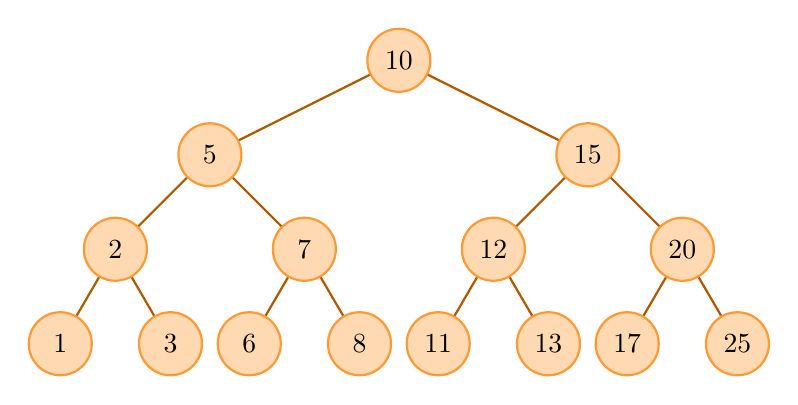
\begin{tikzpicture}[
        sibling distance=12mm,
        level distance=12mm,
        every node/.style={circle, draw=orange!80, fill=orange!30, thick, minimum size=8mm},
        edge from parent/.style={draw=orange!70!black, thick},
        level 1/.style={sibling distance=48mm},
        level 2/.style={sibling distance=24mm},
        level 3/.style={sibling distance=14mm},
        level 4/.style={sibling distance=10mm}
    ]
    
    \node {10}
        child {node {5}
            child {node {2}
                child {node {1}}
                child {node {3}}
            }
            child {node {7}
                child {node {6}}
                child {node {8}}
            }
        }
        child {node (del) {15}
            child {node {12}
                child {node {11}}
                child {node {13}}
            }
            child {node {20}
                child {node {17}}
                child {node {25}}
            }
        };
    \end{tikzpicture}

    \vspace{1em}
    \textbf{Deleting node 15 (Replace with in-order successor 17)}
    \vspace{1em}

    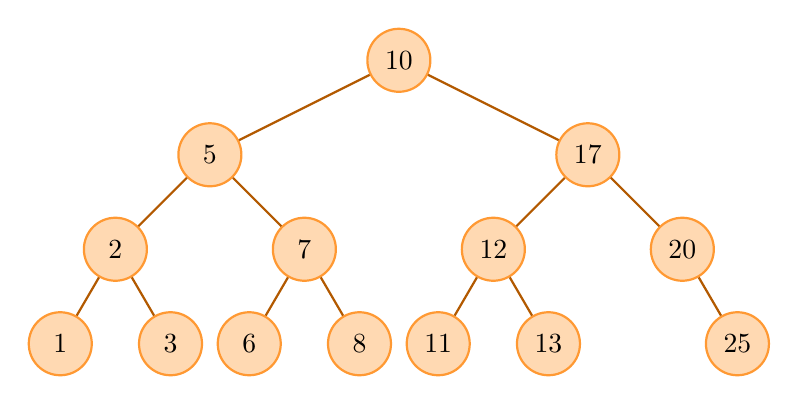
\begin{tikzpicture}[
        sibling distance=12mm,
        level distance=12mm,
        every node/.style={circle, draw=orange!80, fill=orange!30, thick, minimum size=8mm},
        edge from parent/.style={draw=orange!70!black, thick},
        level 1/.style={sibling distance=48mm},
        level 2/.style={sibling distance=24mm},
        level 3/.style={sibling distance=14mm},
        level 4/.style={sibling distance=10mm}
    ]

    \node (root2) {10}
        child {node {5}
            child {node {2}
                child {node {1}}
                child {node {3}}
            }
            child {node {7}
                child {node {6}}
                child {node {8}}
            }
        }
        child {node {17}
            child {node {12}
                child {node {11}}
                child {node {13}}
            }
            child {node {20}
                child[missing]
                child {node {25}}
            }
        };
    \end{tikzpicture}

\end{center}
\subsubsection*{Pseudocode}
\begin{verbatim}
def delete(value, current_node):
    if value < current_node.value:
        current_node.left = delete(value, current_node.left)
    elif value > current_node.value:
        current_node.right = delete(value, current_node.right)
    else:
        # Node with only one child or no child
        if current_node.left is None:
            return current_node.right
        elif current_node.right is None:
            return current_node.left
        # Node with two children
        temp = find_min(current_node.right)
        current_node.value = temp.value
        current_node.right = delete(temp.value, current_node.right)
    return current_node
\end{verbatim}

\subsubsection*{Finding Minimum}
\begin{verbatim}
def find_min(node):
    while node.left is not None:
        node = node.left
    return node
\end{verbatim}

\subsubsection*{Example}
Deleting node with value 21 (has two children):

\begin{verbatim}
         21
        /  \
      14    25
            /
          24
→ Minimum in right subtree: 24
→ Replace 21 with 24
→ Delete 24 from right subtree
\end{verbatim}

This preserves the BST structure while effectively removing the original node.


\end{document}

Don't create any notes yet I will give transcript od subsequent lectures and then we will create notes at once